%\documentclass[a4paper]{article}
%\usepackage[T1,T2A]{fontenc}
%\usepackage[utf8]{inputenc}
%\usepackage[english,russian]{babel}
%\usepackage{booktabs}
%\usepackage{color,colortbl}
%\usepackage{amsmath}
%\usepackage{amsfonts}
%\usepackage{amssymb}
%\usepackage{makeidx}
%\usepackage{tikz}
%\usetikzlibrary{graphs}
%\usepackage{graphicx}
%\definecolor{darkishgreen}{RGB}{39,203,22}
%\definecolor{LightCyan}{rgb}{0.88,1,1}
%\definecolor{Gray}{gray}{0.9}
%\definecolor{lightRed}{RGB}{230,170,150}
%\definecolor{modRed}{RGB}{230,82,90}
%\definecolor{strongRed}{RGB}{230,6,6}

%\usepackage[english,russian]{babel}

%\begin{document}


\section{Лабораторная работа №2.\newline Системы счисления}

Цель работы:
\begin{enumerate}
    \item Понять принципы позиционной системы счисления.
    \item Научиться переводить числа из одной системы в другую.
    \item Уметь производить арифметические действия над числами, представленными в различных системах счисления.
\end{enumerate}

\subsection{Теоретические основы}

Под системой счисления принято понимать совокупность приемов записи чисел. Условные знаки, которые при этом применяются, называют цифрами. В некоторых системах счисления кроме цифр могут использоваться специальные символы. Таким образом, в системах счисления числа записываются как последовательность цифр или специальных символов. Системы счисления подразделяются на позиционные и непозиционные. В непозиционной системе счисления значение цифры не зависит от ее положения в записи числа. К непозиционной системе счисления относится, так называемая, Римская система счисления. Например, возьмем число XXX из Римской системы счисления. В данном числе цифра X в любом месте означает число десять. В позиционных системах счисления значение каждой цифры зависит от ее положения (позиции) в ряду цифр, изображающих это число. Например. В числе 999 (десятичная система счисления) первая справа цифра 9 означает количество единиц, содержащихся в числе, вторая - количество десятков, третья - количество сотен. Принимая за основание системы различные числа можно получить соответствующие системы счисления. Число Рединиц одного разряда, объединяемых в единицу более старшего разряда, называют основанием позиционной системы счисления, а сама система называется Р-ичной. Поэтому для записи произвольного числа в какой-либо позиционной системе счисления достаточно иметь Р различных цифр. Таким образом, любая позиционная система с любым целым основанием P (при P>1) использует Р различных цифр а, которые обозначают последовательный ряд чисел от 0 и кончая числом Р-1.

Число записывается в виде последовательности Р-ичных цифр, которая разделена точкой на целую и дробную части. Если каждый из символов $а_{n}, a_{n-1},\dots,a_{1}, a_{0}, a_{-1}, \dots,a_{m}$ означает некоторую Р-ичную цифру, то запись числа имеет вид $а_{n}, a_{n-1},\dots,a_{1}, a_{0},a_{-1}, \dots,a_{m}$. Каждой цифре из этой последовательности принято определенное значение. Цифра, стоящая в некотором разряде, имеет значение в Р раз большее того, которое она имела бы в разряде с номером, меньшим на
1. И наоборот, в Р раз меньше того, которое она имела бы в разряде с номером, большим на 1.

\subsubsection{Позиционные системы счисления}

Как было сказано, количество различных цифр, применяемых в позиционной системе счисления, называют ее основанием. Принимая за основание системы различные числа можно получить соответствующие системы счисления. К позиционной системе счисления, получившим наибольшее распространение, относятся десятичная, двоичная, восьмеричная и шестнадцатеричная системы счисления. Для того, чтобы отличать в какой системе представлено то или иное число, в дальнейшем будем записыватьчисло с указанием используемой системы счисления. Например, 375ю - число 375 в десятичной системе счисления, а число 3758 - число 375 в восьмеричной системе счисления.

\textbf{Десятичная система счисления}

Это наиболее широко распространенная система счисления, которая использует 10 различных базисных цифр для представления любой величины. При записи чисел в десятичной системе счисления используются символы 0, 1, 2, 3, 4, 5, 6, 7, 8, 9.

Несмотря на простоту и привычность десятичной системы счисления, использование ее при передачи информации в вычислительных машинах представляется неудобной и технически не экономичной. Поэтому при организации вычислительных процессов в ЭВМ используются системы счисления с другими основаниями.

\textbf{Двоичная система счисления}

Большинство элементов, из которых строится ЭВМ, по своей физической природе могут находиться лишь в одном из двух состояний. Такие элементы называются двухпозиционными. Одно из устойчивых состояний элемента принимается за изображение цифры 0, а другое за изображение цифры 1. С помощью двухпозиционных элементов легко изображаются разряды двоичного числа. Поэтому двоичная система счисления имеет преимущества, и она оказывается очень удобной для применения в ЭВМ. Двоичная система счисления имеет только две цифры: 0 и 1. Это минимальное количество цифр, которое может быть принято в системе счисления. Как и в десятичной системе счисления, в двоичной системе для отделения дробной части от целой используется точка, а перед отрицательным числом ставиться минус (-): $101.1_{2}, 1.001_{2}, -101_{2}$.

\textbf{Восьмеричная система счисления}

В цифровых схемах и электронных системах получила распространение восьмеричная система счисления. Данная система удобна тем, что восьмеричная запись какого-либо числа в три раза короче его двоичной записи. В данной системе счисления коэффициенты принимают восемь различных значений - 0, 1, 2, 3, 4, 5, 6, 7.
Поэтому каждый восьмеричный символ может быть представлен трехбитовым числом. Этих чисел восемь, как и символов в восьмеричной системе счисления. Как и в рассмотренных системах счисления, в восьмеричной системе используются дробные и отрицательные числа: $7.35_{8},- 5.001_{8}, 345.67_{8}$.

\textbf{Шестнадцатеричная система счисления}

Для систем счисления с основанием больше «10», арабских цифр для представления чисел не хватит. Поэтому в этих случаях дополнительно вводят специальные символы. К таким системам счисления относится шестнадцатеричная система счисления.В шестнадцатеричной системе счисления используют 16 базисных символов: 0, 1, 2, 3, 4, 5, 6, 7, 8, 9, А, В, С, D, Е, F. Выбор шестнадцатеричной системы счисления обуславливается что эту систему можно использовать как средство сокращенной записи четырехзначного двоичного числа. Следует помнить, что шестнадцатеричные и восьмеричные числа - это только способ представления двоичных чисел. Для представления дробных чисел и отрицательных шестнадцатеричных чисел используется, соответственно, точка и знак минуса (-): $-AB_{16}; 1036.F_{16};FF.13_{16}$.

\subsubsection{Перевод чисел в позиционных системах счисления}

Для перевода целого десятичного числа в другую систему счисления, необходимо разделить исходное число на основание системы счисления, в которое оно переводится. При этом надо определять остатки от деления. Остаток первого деления является значением младшего разряда. Затем полученное частное делится на выбранное основание. Процедуру деления продолжают до тех пор, пока частное не станет меньше делителя, т.е. основания системы счисления, в которую осуществляется перевод. Значение последнего частного будет наибольшим разрядом, т.е. запись нового числа производится в обратном порядке: от частного к первому остатку, используя все промежуточные остатки. При переводе в шестнадцатеричную систему счисления остатки, значения которых больше 9, необходимо заменить соответствующими буквенным эквивалентом: 10 - А, 11 - В, 12 - С, 13 - D, 14 -Е, 15 -F.

Пример перевода десятичного числа 95:

В двоичную систему счисления $95_{10}=1011111_{2}$
\begin{figure}[h]
\center{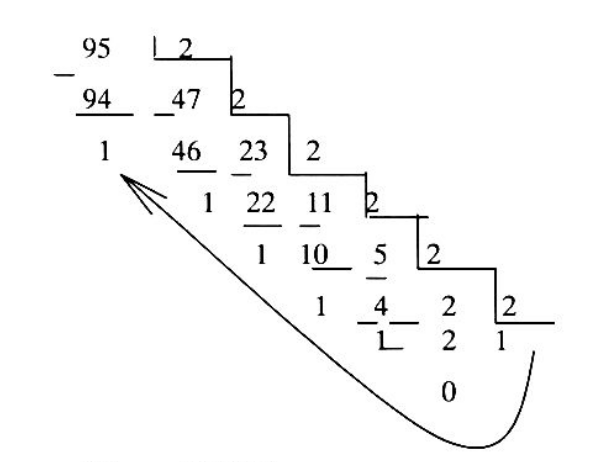
\includegraphics[width=128pt]{dectobin.png}
  \label{ris:dectobin}}
\end{figure}

В восьмиричную систему счисления $95_{10}=137_{8}$
\begin{figure}[h]
\center{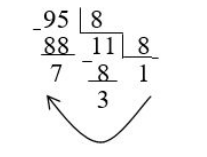
\includegraphics[width=64pt]{dectooct.png}
  \label{ris:dectooct}}
\end{figure}

В шестнадцатиричную систему счисления $95_{10}=5F_{16}$
\begin{figure}[h]
\center{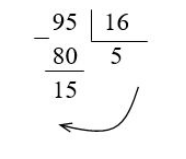
\includegraphics[width=64pt]{dectohex.png}
  \label{ris:dectohex}}
\end{figure}

При переводе правильных десятичных дробей, необходимо умножить значение этой дроби на основание системы счисления, в которую осуществляется перевод. Значение целой части результата первого умножения присваивается старшему разряду дробной части. Затем целая часть не рассматривается и производится следующее умножение дробной части. Процедуру умножения повторяют до тех пор, пока результат умножения не будет равен целому числу и этот результат будет младшим разрядом, либо не будет достигнута требуемая точность.

Пример перевода десятичного числа 0.36:

В двоичную систему счисления $0.36_{10}=0.0101_{2}$
\begin{figure}[h]
\center{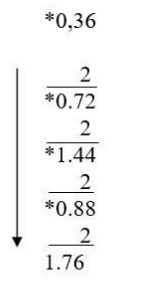
\includegraphics[width=64pt]{fdectobin.png}
  \label{ris:fdectobin}}
\end{figure}

В восьмиричную систему счисления $0.36_{10}=0.2702_{8}$

\begin{figure}[h]
\center{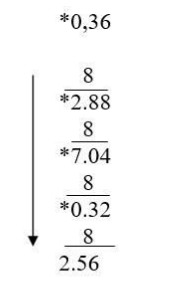
\includegraphics[width=64pt]{fdectooct.png}
  \label{ris:fdectooct}}
\end{figure}

В шестнадцатиричную систему счисления $0.36_{10}=0.5C28_{16}$

\begin{figure}[h]
\center{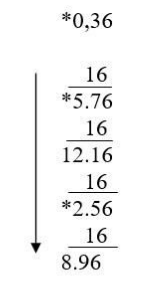
\includegraphics[width=64pt]{fdectohex.png}
  \label{ris:fdectohex}}
\end{figure}

Для перевода неправильной десятичной дроби, необходимо перевести отдельно дробную и целую часть, а полученные результаты сложить. Например, перевести в двоичную систему счисления неправильную десятичную дробь 14.375.
$$14_{10}=1110_{2} 0.375_{10}=0.011_{2} 14.375_{10}=1110.011_{2}$$

\subsubsection{Перевод в десятичную систему счисления}
Для перевода из любой позиционной системы счисления в десятичную систему счисления необходимо записать это число в виде суммы:
$$x = \sum^{n+m}_{i=1}(a_{i}*p^{n-i})$$
где Р --- основание системы из которой осуществляется перевод;\newline
а --- число, соответствующее базисной цифре Р-ичной системы счисления;\newline
n --- число цифр в целой части, m - число цифр в дробной части.\newline
Например, перевести число $110.101_{2}$ из двоичной системы счисления в десятичную:
$$110.101_{2} = 1 * 2^{2} + 1 * 2^{1} + 0 + 1 * 2^{-2} + 1 * 2^{-3} = 6.625_{10}$$

\subsubsection{Перевод из двоичной системы счисления в восьмеричную и шестнадцатеричную}

Основания восьмеричной и шестнадцатеричной систем счисления (q) являются степенью двоичной системы $(р):q=p$, где к --- целое число, равное 3 для восьмеричной системы счисления и 4 для шестнадцатеричной. Поэтому перевод из двоичной системы осуществляется разбиением двоичного числа на группы по три цифры в каждой для восьмеричной и по четыре для шестнадцатеричной. Отчет ведется от точки разделяющей целую часть от дробной в обе стороны. Затем каждая группа заменяется соответствующей цифрой из соответствующих систем счисления(см. табл. \ref{tab:octhex}). Недостающие биты двоичного числа дополняются нулями: впереди - для целой части и в конце - для дробной части. Например, необходимо перевести двоичное число 1010001110.00111 в восьмеричное и шестнадцатеричное число:
\begin{itemize}
  \item в восьмеричное $1010001110.00111_{2} = 001 010 001 100.001 110_{2} = 1214.16_{8}$
  \item в шестнадцатеричное $1010001110.00111_{2} = 0010 1000 1100.0011 1000_{2} = 28С.38_{16}$
\end{itemize}

\begin{table}[h]
  \caption{Соответствие цифр в разных системах счисления}
  \begin{center}\label{tab:octhex}
    \begin{tabular}{|c|c|c|}
      \hline
     Символы & k - 3 & k - 4 \\
     \hline
      0 & 000 & 0000 \\
      1 & 001 & 0001 \\
      2 & 010 & 0010 \\
      3 & 011 & 0011 \\
      4 & 100 & 0100 \\
      5 & 101 & 0101 \\
      6 & 110 & 0110 \\
      7 & 111 & 0111 \\
      8 &     & 1000 \\
      9 &     & 1001 \\
      A &     & 1010 \\
      B &     & 1011 \\
      C &     & 1100 \\
      D &     & 1101 \\
      E &     & 1110 \\
      F &     & 1111 \\
      \hline
     \end{tabular}
  \end{center}
\end{table}

\subsubsection{Перевод в двоичную систему счисления из восьмеричной и шестнадцатеричной}
Для перевода в двоичную систему из восьмеричной или шестнадцатеричной системы счисления необходимо каждое число заменить двоичным эквивалентом (см. табл. \ref{tab:octhex}).

\subsubsection{Перевод из восьмеричной системы в шестнадцатеричную}
Для перевода из восьмеричной системы счисления в шестнадцатеричную систему счисления необходимо представить число в виде двоичного числа. Затем объединить в группы по 4 бита и заменить соответствующим числом из шестнадцатеричной системы счисления (см. табл. \ref{tab:octhex})

\subsubsection{Перевод из шестнадцатеричной системы в восьмеричную}
Для перевода из шестнадцатеричной системы счисления в восьмеричную необходимо представить число в виде двоичного числа. Затем объединить в группы по 3 бита и заменить соответствующим числом из восьмеричной системы счисления (см. табл. \ref{tab:octhex}).

\subsubsection{Арифметические действия в позиционных системах счисления}
Арифметические действия (сложение, вычитание, умножение и деление) над числами в восьмеричной и шестнадцатеричной системах счисления выполняются с использованием таблиц сложения и умножения подобно тому, как это делается в десятичной системе счисления. Таблицы \ref{tab:octsum} и \ref{tab:octmul} предназначены для выполнения сложения и умножения --- в восьмеричной системе счисления, а таблицы \ref{tab:hexsum} и \ref{tab:hexmul} - в шестнадцатеричной системе счисления. Ниже приведены примеры сложения и умножения в различных системах счисления.

\begin{table}[h]
  \caption{Сложение в восьмеричной системе}
  \begin{center}\label{tab:octsum}
\begin{tabular}{|c|c|c|c|c|c|c|c|}
  \hline
  + & 1 & 2 & 3 & 4 & 5 & 6 & 7\tabularnewline
\hline
1 & 2 & 3 & 4 & 5 & 6 & 7 & 10\tabularnewline
\hline
2 & 3 & 4 & 5 & 6 & 7 & 10 & 11\tabularnewline
\hline
3 & 4 & 5 & 6 & 7 & 10 & 11 & 12\tabularnewline
\hline
4 & 5 & 6 & 7 & 10 & 11 & 12 & 13\tabularnewline
\hline
5 & 6 & 7 & 10 & 11 & 12 & 13 & 14\tabularnewline
\hline
6 & 7 & 10 & 11 & 12 & 13 & 14 & 15\tabularnewline
\hline
7 & 10 & 11 & 12 & 13 & 14 & 15 & 16\tabularnewline
                                  \hline
\end{tabular}
\end{center}
\end{table}

\begin{table}[h]
  \caption{Умножение в восьмеричной системе}
  \begin{center}\label{tab:octmul}
\begin{tabular}{|c|c|c|c|c|c|c|c|}
\hline
{*} & 1 & 2 & 3 & 4 & 5 & 6 & 7\tabularnewline
\hline
1 & 1 & 2 & 3 & 4 & 5 & 6 & 7\tabularnewline
\hline
2 & 2 & 4 & 6 & 10 & 12 & 14 & 16\tabularnewline
\hline
3 & 3 & 6 & 11 & 14 & 17 & 22 & 25\tabularnewline
\hline
4 & 4 & 10 & 14 & 20 & 24 & 30 & 34\tabularnewline
\hline
5 & 5 & 12 & 17 & 24 & 31 & 36 & 43\tabularnewline
\hline
6 & 6 & 14 & 22 & 30 & 36 & 44 & 52\tabularnewline
\hline
7 & 7 & 16 & 25 & 34 & 43 & 52 & 61\tabularnewline
\hline
\end{tabular}
\end{center}
\end{table}

\begin{table}[h!]
  \caption{Сложение в шестнадцатеричной системе}
  \begin{center}\label{tab:hexsum}
\begin{tabular}{|c|c|c|c|c|c|c|c|c|c|c|c|c|c|c|c|}
\hline
+ & 1 & 2 & 3 & 4 & 5 & 6 & 7 & 8 & 9 & A & B & C & D & E & F\tabularnewline
\hline
1 & 2 & 3 & 4 & 5 & 6 & 7 & 8 & 9 & A & B & C & D & E & F & 10\tabularnewline
\hline
2 & 3 & 4 & 5 & 6 & 7 & 8 & 9 & A & B & C & D & E & F & 10 & 11\tabularnewline
\hline
3 & 4 & 5 & 6 & 7 & 8 & 9 & A & B & C & D & E & F & 10 & 11 & 12\tabularnewline
\hline
4 & 5 & 6 & 7 & 8 & 9 & A & B & C & D & E & F & 10 & 11 & 12 & 13\tabularnewline
\hline
5 & 6 & 7 & 8 & 9 & A & B & C & D & E & F & 10 & 11 & 12 & 13 & 14\tabularnewline
\hline
6 & 7 & 8 & 9 & A & B & C & D & E & F & 10 & 11 & 12 & 13 & 14 & 15\tabularnewline
\hline
7 & 8 & 9 & A & B & C & D & E & F & 10 & 11 & 12 & 13 & 41 & 15 & 16\tabularnewline
\hline
8 & 9 & A & B & C & D & E & F & 10 & 11 & 12 & 13 & 14 & 15 & 16 & 17\tabularnewline
\hline
9 & A & B & C & D & E & F & 10 & 11 & 12 & 13 & 14 & 15 & 16 & 17 & 18\tabularnewline
\hline
A & B & C & D & E & F & 10 & 11 & 12 & 13 & 14 & 15 & 16 & 17 & 18 & 19\tabularnewline
\hline
B & C & D & E & F & 10 & 11 & 12 & 13 & 14 & 15 & 16 & 17 & 18 & 19 & 1A\tabularnewline
\hline
C & D & E & F & 10 & 11 & 12 & 13 & 14 & 15 & 16 & 17 & 18 & 19 & 1A & 1B\tabularnewline
\hline
D & E & F & 10 & 11 & 12 & 13 & 14 & 15 & 16 & 17 & 18 & 19 & 1A & 1B & 1C\tabularnewline
\hline
E & F & 10 & 11 & 12 & 13 & 14 & 15 & 16 & 17 & 18 & 19 & 1A & 1B & 1C & 1D\tabularnewline
\hline
F & 10 & 11 & 12 & 13 & 14 & 15 & 16 & 17 & 18 & 19 & 1A & 1B & 1C & 1D & 1E\tabularnewline
\hline
\end{tabular}
\end{center}
\end{table}

\begin{table}[h!]
  \caption{Умножение в шестнадцатеричной системе}
  \begin{center}\label{tab:hexmul}
\begin{tabular}{|c|c|c|c|c|c|c|c|c|c|c|c|c|c|c|c|}
\hline
{*} & 1 & 2 & 3 & 4 & 5 & 6 & 7 & 8 & 9 & A & B & C & D & E & F\tabularnewline
\hline
1 & 1 & 2 & 3 & 4 & 5 & 6 & 7 & 8 & 9 & A & B & C & D & E & F\tabularnewline
\hline
2 & 2 & 4 & 6 & 8 & A & C & E & 10 & 12 & 14 & 16 & 18 & 1A & 1C & 1E\tabularnewline
\hline
3 & 3 & 6 & 9 & C & F & 12 & 15 & 18 & 1B & 1E & 21 & 24 & 27 & 2A & 2D\tabularnewline
\hline
4 & 4 & 8 & C & 10 & 14 & 18 & 1C & 20 & 24 & 28 & 2C & 30 & 34 & 38 & 3C\tabularnewline
\hline
5 & 5 & A & F & 14 & 19 & 1E & 23 & 28 & 2D & 32 & 37 & 3C & 41 & 46 & 4B\tabularnewline
\hline
6 & 6 & C & 12 & 18 & 1E & 24 & 2A & 30 & 36 & 3C & 42 & 48 & 4E & 54 & 5A\tabularnewline
\hline
7 & 7 & E & 15 & 1C & 23 & 2A & 31 & 38 & 3F & 46 & 4D & 54 & 5B & 62 & 69\tabularnewline
\hline
8 & 8 & 10 & 18 & 20 & 28 & 30 & 38 & 40 & 48 & 50 & 58 & 60 & 68 & 70 & 78\tabularnewline
\hline
9 & 9 & 12 & 1B & 24 & 2D & 36 & 3F & 48 & 51 & 5A & 63 & 6C & 75 & 7E & 87\tabularnewline
\hline
A & A & 14 & 1E & 28 & 32 & 3C & 46 & 50 & 5A & 64 & 6E & 78 & 82 & 8C & 96\tabularnewline
\hline
B & B & 16 & 21 & 2C & 37 & 42 & 4D & 58 & 63 & 6E & 79 & 84 & 8F & 9A & A5\tabularnewline
\hline
C & C & 18 & 24 & 30 & 3C & 48 & 54 & 60 & 6C & 78 & 84 & 90 & 9C & A8 & B4\tabularnewline
\hline
D & D & 1A & 27 & 34 & 41 & 4E & 5B & 68 & 75 & 82 & 8F & 9C & A9 & B6 & C3\tabularnewline
\hline
E & E & 1C & 2A & 38 & 46 & 54 & 62 & 70 & 7E & 8C & 9A & A8 & B6 & C4 & D2\tabularnewline
\hline
F & F & 1E & 2D & 3C & 4B & 5A & 69 & 78 & 87 & 96 & A5 & B4 & C3 & D2 & E1\tabularnewline
\hline
\end{tabular}
\end{center}
\end{table}


\newpage*
\subsection{Задание на лабораторную работу}

Для выполнения работы необходимо:
\begin{enumerate}
  \item Изучить теоретический материал
  \item Выполнить все задания
  \item Оформить отчет по лабораторной работе
\end{enumerate}

\subsubsection{Порядок выполнения работы}

Для выполнения работы по системам счисления необходимо изучить теоретический материал и из таблицы \ref{tab:task2_1} выбрать числовые данные и выполнить перевод из одной системы счисления в другую по следующей схеме:
\begin{enumerate}
  \item Перевод из десятичной системы в двоичную
  \item Перевод из десятичной системы в восьмеричную
  \item Перевод из десятичной системы в шестнадцатеричную
  \item Перевод из двоичной системы в восьмеричную
  \item Перевод из двоичной системы в десятичную
  \item Перевод из двоичной системы в шестнадцатеричную
  \item Перевод из восьмеричной системы в двоичную
  \item Перевод из восьмеричной системы в десятичную
  \item Перевод из восьмеричной системы в шестнадцатеричную
  \item Перевод из шестнадцатеричной системы в двоичную
  \item Перевод из шестнадцатеричной системы в восьмеричную
  \item Перевод из шестнадцатеричной системы в десятичную
\end{enumerate}
Из таблицы \ref{tab:task2_2} в соответствии с номером варианта необходимо выбрать данные для проведения арифметических действий в системах счисления по следующей схеме:
\begin{enumerate}
  \item Произвести сложение в восьмеричной системе
  \item Произвести умножение в восьмеричной системе
  \item Произвести сложение в шестнадцатеричной системе
  \item Произвести умножение в шестнадцатеричной системе
\end{enumerate}

\begin{sidewaystable}
  \caption{Задание 1}
  \begin{center}\label{tab:task2_1}
\begin{tabular}{|c|c|c|c|c|c|c|c|c|c|c|c|c|}
\hline
Вариант & 1 & 2 & 3 & 4 & 5 & 6 & 7 & 8 & 9 & 10 & 11 & 12\tabularnewline
\hline
1 & 7.5 & 32.01 & 23.56 & 1011.1010 & 110101l.01 & 110101.01001 & 12.5 & 44.55 & 34.56 & 1A.23 & 24.57 & AC.C1\tabularnewline
\hline
2 & 72.12 & 80.97 & 42.55 & 1101.110 & 10101010.10 & 11011001.111 & 12.4 & 23.44 & 3.24 & 1C.23 & 67.23 & 5F.5D\tabularnewline
\hline
3 & 12.34 & 41.2 & 15.43 & 110111.11 & 110.1100 & 110011.0011 & 51.4 & 23.56 & 54.63 & 17.23 & 53.74 & 6A.F5\tabularnewline
\hline
4 & 56.3 & 41.67 & 17.87 & 11001.101 & 111.0001 & 1000111.111 & 51.6 & 34.56 & 23.56 & 19.12 & 83.43 & C6.3D\tabularnewline
\hline
5 & 22.4 & 78.2 & 5.66 & 100000.111 & 10101.0001 & 1110001.001 & 32.4 & 32.45 & 76.54 & FF.12 & 86.35 & 1D.2D\tabularnewline
\hline
6 & 51.61 & 56.2 & 57.84 & 1110011.10 & 101001.101 & 1111100.011 & 76.54 & 56.43 & 64.34 & 12.51 & 26.57 & 1F.F2\tabularnewline
\hline
7 & 2.5 & 53.1 & 2.45 & 101010.10 & 100111.01 & 010010.001 & 23.64 & 45.64 & 34.56 & 89.31 & AF.FF & 13.AF\tabularnewline
\hline
8 & 67.15 & 5.2 & 64.88 & 1010.001 & 100100.100 & 1001001.001 & 12.34 & 1.34 & 32.43 & AF.43 & FD.CD & FA.2D\tabularnewline
\hline
9 & 66.6 & 12.67 & 99.12 & 1010001 & 101010.010 & 101000101 & 12.45 & 16.74 & 71.55 & 12.AF & A5.F5 & 6A.7D\tabularnewline
\hline
10 & 6.66 & 1.3 & 45.8 & 11001.0101 & 111111.111 & 1011111.111 & 43.43 & 56.42 & 16.41 & 34.17 & A5.56 & 7D.9A\tabularnewline
\hline
11 & 1.23 & 5.7 & 23.5 & 10001.111 & 111.1101 & 1001110 & 66.66 & 54.67 & 64.67 & 1C.24 & AF.23 & 87.43\tabularnewline
\hline
12 & 3.21 & 8.6 & 13.12 & 100110.11 & 10001.1010 & 110010000.1 & 77.77 & 65.67 & 23.62 & BA.2A & 12.FF & AF.FA\tabularnewline
\hline
13 & 32.1 & 45.85 & 13.09 & 11001000 & 1.01001 & 11001011 & 42.56 & 42.45 & 34.52 & FF.AA & 53.FF & B6.B5\tabularnewline
\hline
14 & 78.12 & 13.67 & 29.45 & 1000.001 & 11.001 & 1011011.111 & 23.56 & 34.54 & 26.23 & 46.FD & 65.FC & B3.F2\tabularnewline
\hline
15 & 12.2 & 66.12 & 42.5 & 1010.001 & 101.011 & 11011010 & 16.71 & 53.54 & 37.53 & 78.32 & 87.AF & 4F.34\tabularnewline
\hline
16 & 76.2 & 67.12 & 75.7 & 1001100.01 & 111.001001 & 1010111 & 71.56 & 65.65 & 23.72 & 56.FA & AF.FA & 5F.B3\tabularnewline
\hline
17 & 1.2 & 34.48 & 34.77 & 1101.01 & 101001.10 & 101010101 & 46.53 & 53.63 & 25.62 & 12.EE & AD.DA & B3.BB\tabularnewline
\hline
18 & 51.5 & 12.78 & 23.56 & 10.10001 & 100100.011 & 100.1001 & 15.36 & 23.54 & 23.53 & 56.34 & CE.DE & BB.BB\tabularnewline
\hline
19 & 15.12 & 23.21 & 34.7 & 11.1111 & 1001010.01101 & 1010.001 & 74.65 & 63.54 & 23.63 & 1C.AF & FE.EE & CC.CC\tabularnewline
\hline
20 & 12.12 & 21.12 & 53.2 & 1011.1 & 1010101010 & 1000.0001 & 23.56 & 55.55 & 22.22 & A1.F1 & AA.AA & FF.FF\tabularnewline
\hline
\end{tabular}
\end{center}
\end{sidewaystable}

\begin{table}[h!]
  \caption{Задание 2}
  \begin{center}\label{tab:task2_2}
\begin{tabular}{|c|c|c|c|c|}
\hline
Вариант & 1 & 2 & 3 & 4\tabularnewline
\hline
1 & 353.56+12.56 & 32.43{*}34.1 & A1+A2 & A1{*}A2\tabularnewline
\hline
2 & 123.456+76.43 & 8{*}8 & C+4 & C{*}4\tabularnewline
\hline
3 & 54+87.38 & 7.7{*}7.7 & F+F & F{*}F\tabularnewline
\hline
4 & 12.45+66.44 & 7{*}7 & FF+F1 & FF{*}F1\tabularnewline
\hline
5 & 112.54+66.44 & 12{*}23 & 22+F & 22{*}F\tabularnewline
\hline
6 & 54.3+65.1 & 0.1{*}0.5 & 4F+C1 & 4F{*}C1\tabularnewline
\hline
7 & 8+8 & 5.5{*}5.5 & 21+21 & 21{*}21\tabularnewline
\hline
8 & 67+54.1 & 2{*}7.3 & 12+13 & 12{*}13\tabularnewline
\hline
9 & 12.32+12.32 & 43{*}12.1 & 16+17 & 16{*}17\tabularnewline
\hline
10 & 77+77.77 & 23{*}12.5 & F1+1D & F1{*}1D\tabularnewline
\hline
11 & 43.23+76 & 23.1{*}3.3 & AC+CA & AC{*}CA\tabularnewline
\hline
12 & 543.1+12.1 & 55{*}55 & DE+E & DE{*}E\tabularnewline
\hline
13 & 12.43+42.34 & 77{*}77 & 1E+E1 & 1E{*}E1\tabularnewline
\hline
14 & 65.2+23.4 & 32{*}23.1 & 11+12 & 11{*}12\tabularnewline
\hline
15 & 12.53+12.12 & 12.65{*}23 & 13+14 & 13{*}14\tabularnewline
\hline
16 & 43+123.123 & 32{*}34.12 & 54+2F & 54{*}2F\tabularnewline
\hline
17 & 53.46+77 & 54.4{*}23.34 & 23+F1 & 23{*}F1\tabularnewline
\hline
18 & 7+7.777 & 23.7{*}34.1 & 12+2F & 12{*}2F\tabularnewline
\hline
19 & 76.3+67.534 & 23.77{*}21.32 & 12+34 & 12{*}34\tabularnewline
\hline
20 & 1.37+1.76 & 23.55{*}34.23 & FA+FF & FA{*}FF\tabularnewline
\hline
\end{tabular}
\end{center}
\end{table}

\newpage
\subsection{Содержание отчета}
\begin{enumerate}
  \item Титульный Лист
  \item Цель работы
  \item Краткие теоретические сведения по теме лабораторной работы
  \item Выполненное задание
  \item Краткий вывод о проделанной работе
\end{enumerate}

\begin{thebibliography}{3}
  \bibitem{kon1}
  Коноплева, И.А. Информационные технологии: Учеб. пособие/ Коноплева И.А., Хохлова И.А., Денисов А.. - 2-е изд. - М.: Проспект, 2014.- 328 с.
\bibitem{zab2}
Забуга, А.А. Теоретические основы информатики: Учеб. пособие/ Забуга А.А. - СПб.: Питер, 2014.- 208 с.: ил.- (Учебное пособие. Стандарт третьего поколения).
\end{thebibliography}

%\end{document}
